\documentclass[final,5p,times,twocolumn,sort&compress]{elsarticle}
\usepackage{amssymb, lipsum}
\usepackage{makecell}
\usepackage{xeCJK}

% useful packages
\usepackage{amsmath}
\usepackage{graphicx}
\usepackage{subfig}
\usepackage[colorlinks=true, allcolors=blue]{hyperref}
\usepackage{float}

\newcommand{\kms}{km\,s$^{-1}$}
\newcommand{\msun}{$M_\odot}
\newcolumntype{x}[1]{>{\centering\arraybackslash\hspace{0pt}}p{#1}}
% appendix
\usepackage[toc,page]{appendix}
\usepackage{etoolbox}
\BeforeBeginEnvironment{appendices}{\clearpage}

\journal{DLMI 2024 spring}
\begin{document}

\begin{frontmatter}

    \title{Deep Learning for Medical Imaging 2024 Spring Midterm Project}
    \author[1,2]{廖致豪 R11625015}
    \address[1]{National Taiwan University, School of Forestry and Resource Conservation, Taipei, Taiwan}
    \address[2]{National Taiwan University, Graduate Institute of Biomedical Electronics and Bioinformatics, Taipei, Taiwan}

    \begin{abstract}
        This report is Prof. Ruey-Feng Chang's deep learning for the medical imaging spring course's midterm project. I was given the assignment of devising a midterm project focusing on Deep Learning in Medical Imaging. A classification system that can predict different types of breast ultrasound images (US) will be implemented via various state-of-the-art (SOTA) CNN models, such as AlexNet, VGG16, GoogLeNet, and ResNet18. In this project, the images will be preprocessed by performing different transformation processes, and normalized by pre-trained ImageNet parameters. All selected SOTA models will be built with best validation accuracy, to build a baseline model, followed by applying advanced techniques, including data augmentation, and architecture modification, to further improve the performance of SOTA models. The result showed that our work is pretty decent, and the self-modified CNN model has the best accuracy.
    \end{abstract}

    \begin{keyword}
        Breast Ultrasound Images \sep  Deep Learning \sep  State-of-the-Art
    \end{keyword}

\end{frontmatter}

%% main text
\section{Introduction}
\label{introduction}
\subsection{Background}
Medical ultrasound (US) imaging has emerged as a prominent tool for breast cancer detection, owing to its simplicity, affordability, and safety. The interpretation of breast ultrasound images has long been crucial in clinical settings. Therefore, employing machine learning classification techniques to swiftly assess breast ultrasound images can greatly aid in clinical decision-making and treatment planning. In this project, we will we will utilize several kinds of machine learning techniques to classify breast US images.

\subsection{Frame The Problem}
The problem in this project is a classic multi-class classification problem:

Given a training set of input-output pairs ${\cal D}_{train} = \{({\mathbf x_n}, y_n)\}_{n=1}^{N}$, and find $f$ such that $f(\mathbf{x})=\hat{y}\sim y,\ y\in\{0,1,2\}\ or\ y\in\{0,2\},\ {\mathbf x} \in \mathbb{R}^{d}$. Then, minimize $\text{err}(\hat{y}, y)$, defined as Mean Absolute Error (MAE) in this project, for a learning algorithm to select $f$ out.

\subsection{Performance Measurement}
This project evaluates the performance of our model by Mean Absolute Error (MAE), we can formulate the equation below (\ref{mae}):

\begin{equation}
    \label{mae}
    MAE=\frac{1}{n}\sum_{i}^{n}|\hat{y}_{i}-y_{i}|
\end{equation}

Where $n$ is the number of labels, $\hat{y}_{i}$ is the $i$-th predicted label, and $y_{i}$ is the i-th true label.

\section{Method}
\subsection{Dataset}
The dataset published online by Al-Dhabyani \emph{et al} \cite{ALDHABYANI2020104863} was used in this project, which comprised 780 images (referred to as BUSI) obtained from 600 women patients, with an average image size of 500 x 500 pixels pixels. The BUSI dataset are categorized into three classes, and there are 133 normal images, 437 malignant masses, and 210 benign tumors. All the training images will be resized to 224 x 224. Figure \ref{fig:BUSI} illustrates examples of breast US imags. To assess the performance of the classification models, common metrics used in medical image studies are employed, such as classification accuracy.

\begin{figure}[H]
    \centering
    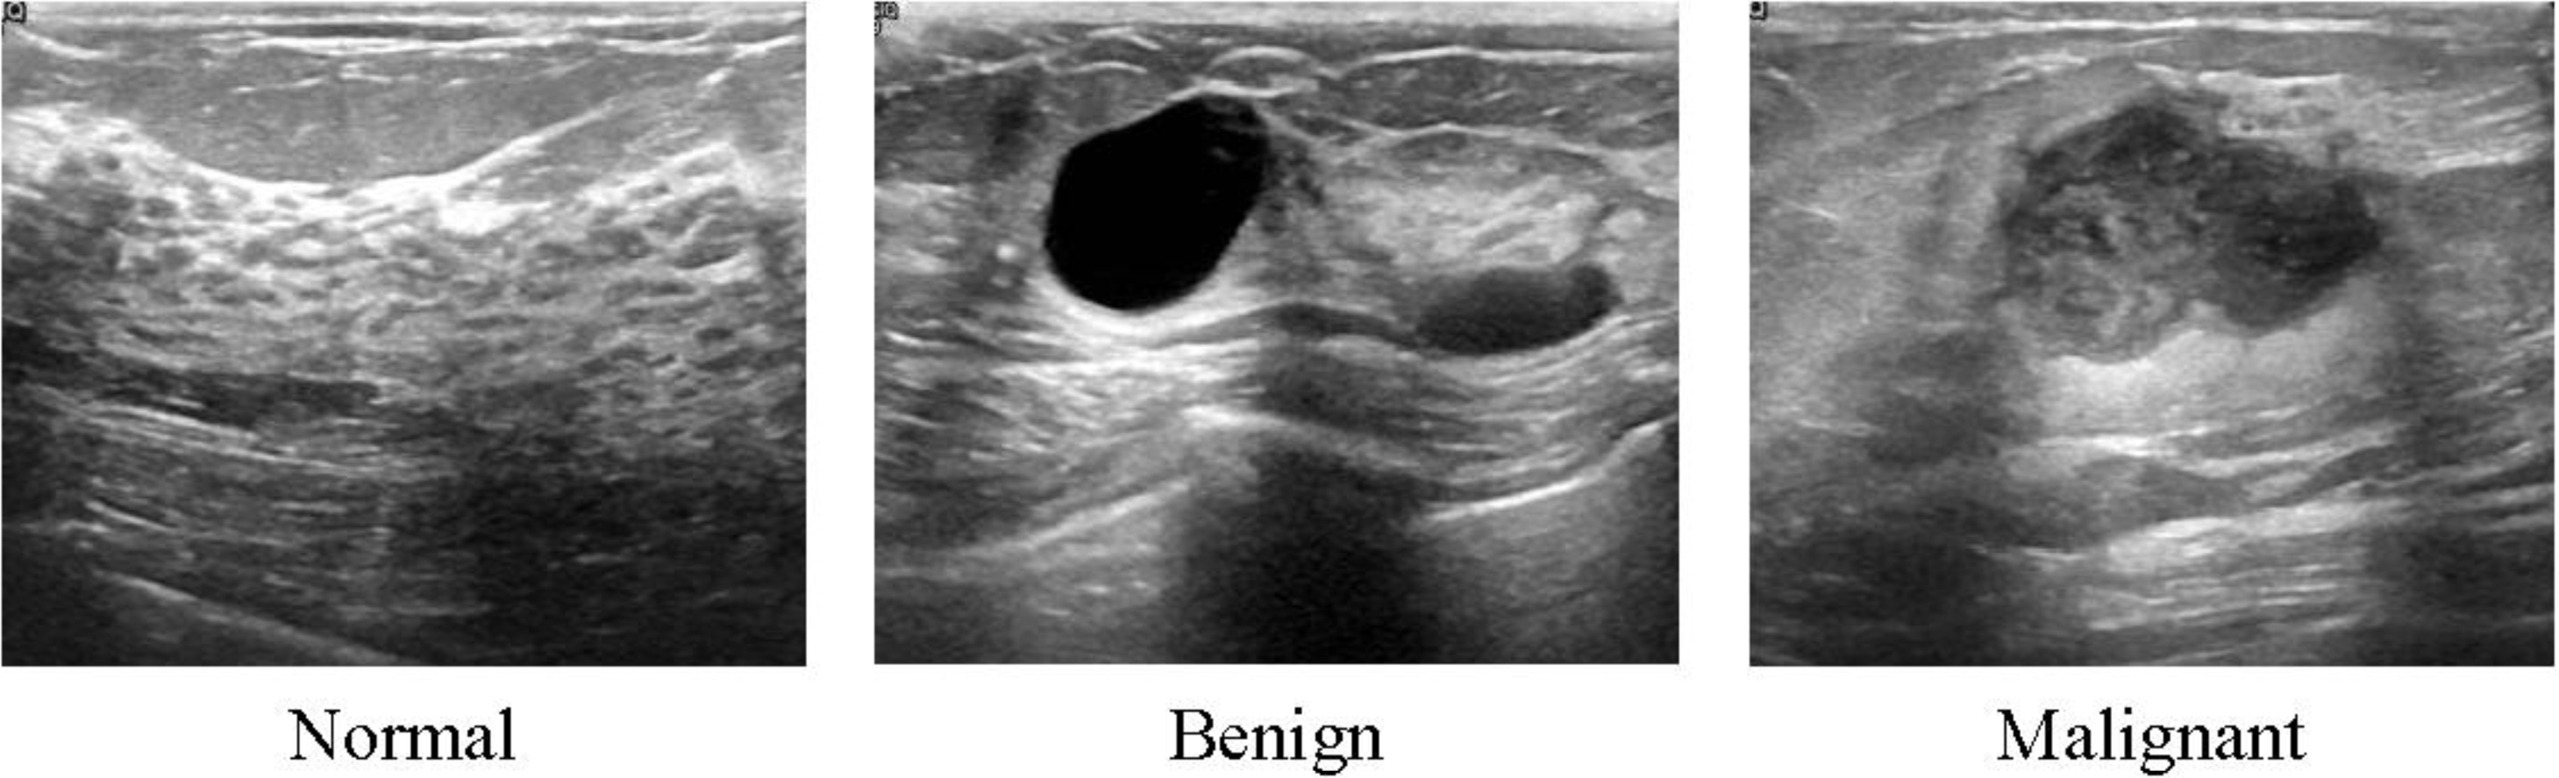
\includegraphics[width=0.45\textwidth]{./img/figure_1.jpg}
    \caption{The samples of breast US images with three different categories.}
    \label{fig:BUSI}
\end{figure}

\subsection{Preprocess}
\subsubsection{Data Augmentation}
Since CNN models are powerful and widely used for image classification tasks, inherently lack rotational invariance. This means that if an image is rotated, even slightly, the network may fail to recognize the object in the image correctly.

To address the data variability and the rotational invariance,  randomly horizontal flip images with a fifty-fifty possibility, followed by randomly rotating the images with default expansion, which means the image size won't be changed, but this helps the network learn to recognize objects from different orientations. By augmenting the data, we introduce variability into the training set, which helps the model learn to generalize better and become more robust to changes in the input data.

\subsubsection{Normalization}
Normalization improves model performance by scaling input features to a similar range, aiding convergence, and preventing gradient explosion or vanishing. It enhances stability, accelerates training, and enables networks to learn efficiently from data, leading to faster convergence and better generalization. The normalization equation can be depicted below (\ref{normaliation}):

\begin{equation}
    \label{normaliation}
    \hat{x}_{i,d}=\frac{x_{i,d}}{max(|x_{1,d}|, |x_{2,d}|,\dots,|x_{n,d}|)}
\end{equation}

Where $\hat{x}_{i,d}$ is the $i$-th row, $d$-th dimension's new feature, $x_{i,d}$ is the $i$-th row, $d$-th dimension's original feature. However, researches suggest \cite{10.1145/3450439.3451867} \cite{kornblith2019better} that employing pre-trained weights from ImageNet provides better performance than randomly initialized weights. Additionally, studies show that architectures trained on ImageNet tend to generalize well. As a result, normalization methods utilize pre-trained weights from ImageNet, integrating mean (0.485, 0.456, 0.406) and standard deviation (0.229, 0.224, 0.225) for feature normalization in this project.

\subsection{Models}
To ensure uniformity in input image dimensions and better accuracy for classification tasks, some popular SOTA CNN models such as AlexNet, VGG16, GoogLeNet, and ResNet18 were selected for training in this project.

\subsubsection{AlexNet}
In our project methodology, we include AlexNet \cite{NIPS2012_c399862d} as the baseline model for our image classification experiments. It's architecture is depicted on Figure \ref{fig:AlexNet_arch}. AlexNet consists of five convolutional layers followed by three fully connected layers, with ReLU activation functions applied after each convolutional and fully connected layer. The architecture is characterized by incorporating max-pooling layers to downsample features and dropout layers to prevent overfitting, and the layers enable the model to automatically learn hierarchical features from raw image data.

During fine-tuning, we typically modify the final fully connected layers of AlexNet to match the number of classes in our dataset. By adopting AlexNet as our baseline model, we establish a benchmark for comparison with more recent and sophisticated architectures. Its relatively simple architecture and well-established training procedures make it a suitable starting point for our experiments.

Additionally, since AlexNet has been extensively studied and widely implemented, it serves as a reference point for evaluating the advancements and performance improvements achieved by newer models.

\begin{figure}[H]
    \centering
    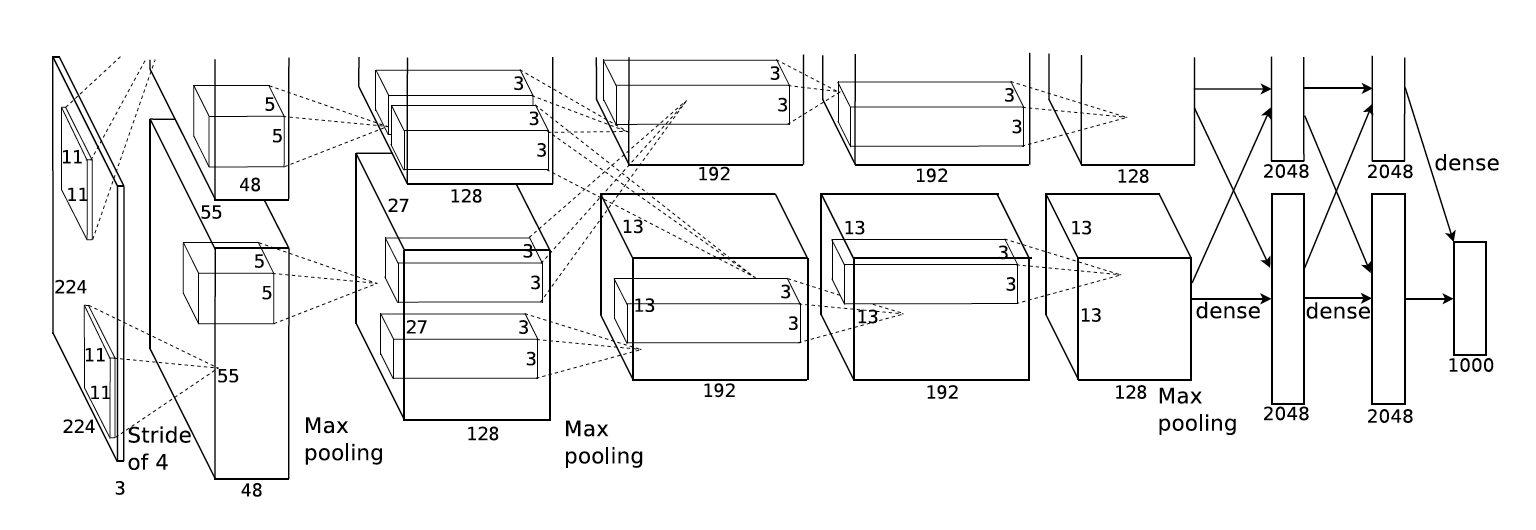
\includegraphics[width=0.45\textwidth]{./img/alexnet.png}
    \caption{The architecture of AlexNet.}
    \label{fig:AlexNet_arch}
\end{figure}

\subsubsection{VGG16}
\begin{figure}[H]
    \centering
    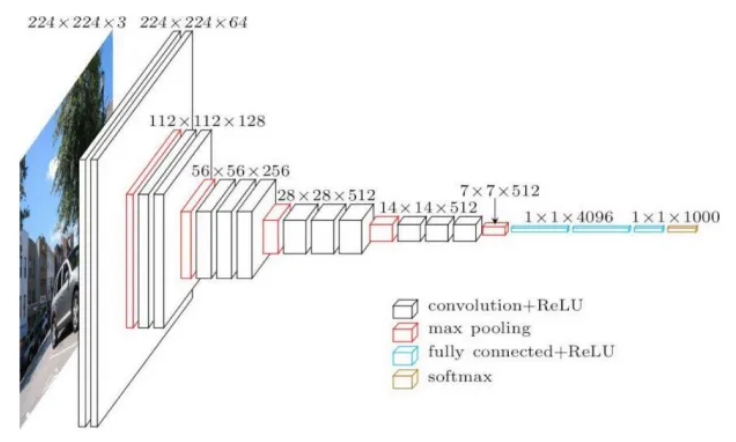
\includegraphics[width=0.45\textwidth]{./img/VGG_arch.jpg}
    \caption{The architecture of VGG16.}
    \label{fig:VGG16_arch}
\end{figure}

The architecture of VGG16 \cite{simonyan2015deep} is depicted on Figure \ref{fig:VGG16_arch}, and is characterized by its simplicity and effectiveness. It consists of 16 layers, including 13 convolutional layers and 3 fully connected layers, all layers are showd on Figure \ref{fig:VGG16_layers}. The convolutional layers are composed of 3x3 filters with a stride of 1 and a padding of 1, followed by max-pooling layers of 2x2 with a stride of 2. This design allows VGG16 to effectively capture hierarchical features from input images while maintaining spatial information.

\begin{figure}[H]
    \centering
    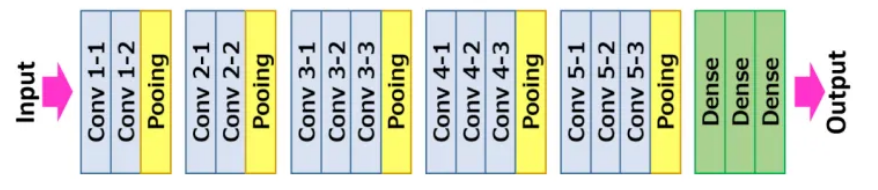
\includegraphics[width=0.45\textwidth]{./img/VGG_layers.jpg}
    \caption{The overall VGG16 layers from input to output.}
    \label{fig:VGG16_layers}
\end{figure}

\subsubsection{GoogLeNet}
GoogLeNet \cite{7298594}, also known as Inception-v1, is notable for its inception modules, which allow for efficient and parallel processing of information at multiple scales. The architecture is characterized by its depth and computational efficiency, achieved through the innovative use of inception modules, which allow for efficient and parallel processing of information at multiple scales. The architecture is showed on Figure \ref{fig:GoogLeNet_arch}.

These modules consist of multiple parallel convolutional layers with different receptive field sizes, including 1x1, 3x3, and 5x5 convolutions, along with max-pooling operations. By incorporating these diverse operations within each inception module, GoogLeNet can capture rich spatial hierarchies of features across different scales.

\begin{figure}[H]
    \centering
    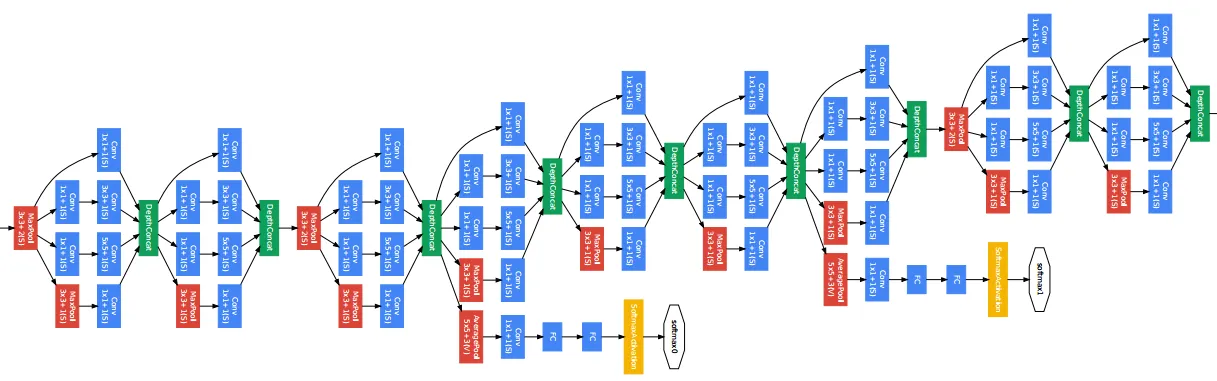
\includegraphics[width=0.45\textwidth]{./img/GoogleNet_arch.png}
    \caption{The architecture of GoogLeNet.}
    \label{fig:GoogLeNet_arch}
\end{figure}

\subsubsection{ResNet18}
The core innovation of ResNet18 lies in the introduction of residual connections, or skip connections, which enable the network to learn residual mappings rather than attempting to directly learn the desired underlying mapping. These skip connections facilitate the flow of gradients during training, mitigating the vanishing gradient problem and allowing for the successful training of very deep networks. ResNet18 specifically consists of 18 layers showed on Figure \cite{7780459}, with a basic building block structure comprising convolutional layers, batch normalization, ReLU activation functions, and residual connections. The network architecture is designed to gradually downsample feature maps while increasing the number of filters, enabling the model to capture increasingly abstract and complex features from input images.

\begin{figure}[H]
    \centering
    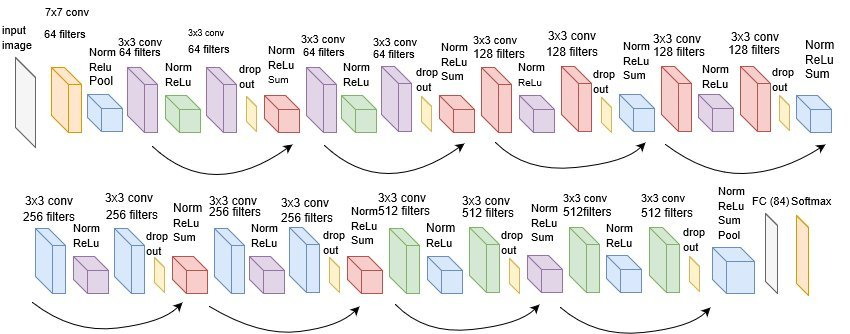
\includegraphics[width=0.45\textwidth]{./img/ResNet18_arch.jpg}
    \caption{The architecture of ResNet18.}
    \label{fig:ResNet18_arch}
\end{figure}

\subsection{Experimental Procedure}
Before initiating the project, we perform manual processing on the raw data, ensuring it conforms to the required format and integrating it into the dataset for subsequent processing stages. Subsequently, we engage in preprocessing the dataset, which involves three primary phases. Initially, we assign true labels to the images based on the structured file names. Then, employing the train\_test\_split function, we segment the data into training, testing, and validation subsets,maintaining proportions of $0.6$, $0.2$, and $0.2$, respectively. Finally, we preserve the filename and label information within the annotation.json file for reference and downstream task processing.

\subsubsection{Build Baseline Models}
After preprocessing, I aim to swiftly establish a rudimentary model to serve as a baseline model for refining and referencing subsequent models. To achieve this,  I opt for AlexNet as the initial baseline model for this purpose. Throughout the model establishment process, no adjustments were made to any parameters until the model was fully constructed. Only then are slight adjustments made to the hyperparameters. Subsequently, subsequent models are then trained using these same hyperparameters, facilitating the establishment of baseline models across various CNN architectures, which can be used as benchmarks for future optimization endeavors.

\section{Result and Discussion}
\label{Result and Discussion}
After applying various data augmentation techniques and modifying the model architectures, the research findings reveal a noticeable improvement in accuracy for most models after optimization. Both during the training and validation phases, it's apparent that all models perform better than AlexNet, achieving accuracies exceeding 70\%. Notably, GoogleNet stands out with an accuracy of 82.05\%.

However, when tested on a private dataset, nearly all models exhibit a significant decline in classification accuracy,  indicating a strong association with evident overfitting. Furthermore, the limited size of the training dataset, comprising fewer than 500 samples, increases the likelihood of encountering issues like early gradient saturation during training.

\begin{table}[H]
    \caption{\label{tab:data accuracy} Model accuracies on public and private datasets.}
    \centering
    \begin{tabular}{|x{60pt}|x{70pt}|x{60pt}|}
        \hline
        Models                                   & Train/Valid(\%) & Test (\%) \\
        \hline
        \hline
        \rule{0pt}{10pt}\makecell[c]{AlexNet}    & 67.95           & 64.10     \\
        \hline
        \rule{0pt}{10pt}\makecell[c]{VGG16}      & 76.92           & 68.59     \\
        \hline
        \rule{0pt}{10pt} \makecell[c]{GoogLeNet} & 82.05           & 73.08     \\
        \hline
        \rule{0pt}{10pt}\makecell[c]{ResNet18}   & 78.85           & 71.79     \\
        \hline
    \end{tabular}
\end{table}

Analyzing the data in the appendix reveals distinct patterns across different models.  In the training process of AlexNet, there are performance plateaus around epoch 40, followed by a potential decline starts to appear. Delve into the data for VGG16, it exhibits promising training curve performance; however, there is a notable rapid increase in validation accuracy early on, suggesting data scarcity issues.

GoogleNet, boasting the highest accuracy, demonstrates relatively stable training but experiences notable validation fluctuations due to limited data, this can be proved from other researches \cite{gheflati2022vision}. Contrastingly, ResNet18 fails to converge, with significant validation loss fluctuations, indicating ineffective learning updates possibly due to inappropriate learning rates, resulting in lower final accuracy.

\section{Conclusion}
\label{Conclusion}
In the initial stage, we established baseline models by adjusting hyperparameters. Subsequently, we enhanced data variability through various data augmentation techniques. During training, we experimented with modifying model architectures to improve accuracy and feature extraction capabilities. Despite these efforts, there are still many areas for improvement. For instance, leveraging masked images provided by the original data to extract feature regions for training, or employing a feature extraction approach where classification precedes training, are avenues for further research and development.

Looking ahead, we aim to explore novel approaches to feature extraction and representation learning. This includes investigating methods such as self-supervised learning, where the model learns to predict certain properties of the input data without explicit supervision, and then fine-tuning the model on the downstream task of interest.

Overall, our journey towards improving model performance is ongoing and multi-faceted. By continuously exploring new techniques and refining existing methodologies, we strive to push the boundaries of what is possible in the field of machine learning and pattern recognition.

% biotex
\bibliographystyle{elsarticle-harv}
\bibliography{reference}

% appendix
\begin{appendices}
    \section{AlexNet}
    \begin{figure}[H]
        \centering
        \includegraphics[width=0.4\textwidth]{./experiment/AlexNet_2024_04_17_21_49_56_DLMI_/log/train_acc_list.png}
        \caption{Accuracy curve of AlexNet training process.}
    \end{figure}
    \begin{figure}[H]
        \centering
        \includegraphics[width=0.4\textwidth]{./experiment/AlexNet_2024_04_17_21_49_56_DLMI_/log/train_loss_list.png}
        \caption{Loss curve of AlexNet training process.}
    \end{figure}
    \begin{figure}[H]
        \centering
        \includegraphics[width=0.4\textwidth]{./experiment/AlexNet_2024_04_17_21_49_56_DLMI_/log/val_acc_list.png}
        \caption{Accuracy curve of AlexNet validation process.}
    \end{figure}
    \begin{figure}[H]
        \centering
        \includegraphics[width=0.4\textwidth]{./experiment/AlexNet_2024_04_17_21_49_56_DLMI_/log/val_loss_list.png}
        \caption{Loss curve of AlexNet validation process.}
    \end{figure}

    \section{VGG16}
    \begin{figure}[H]
        \centering
        \includegraphics[width=0.4\textwidth]{./experiment/VGG_2024_04_17_21_25_32_DLMI_/log/train_acc_list.png}
        \caption{Accuracy curve of VGG16 training process.}
    \end{figure}
    \begin{figure}[H]
        \centering
        \includegraphics[width=0.4\textwidth]{./experiment/VGG_2024_04_17_21_25_32_DLMI_/log/train_loss_list.png}
        \caption{Loss curve of VGG16 training process.}
    \end{figure}
    \begin{figure}[H]
        \centering
        \includegraphics[width=0.4\textwidth]{./experiment/VGG_2024_04_17_21_25_32_DLMI_/log/val_acc_list.png}
        \caption{Accuracy curve of VGG16 validation process.}
    \end{figure}
    \begin{figure}[H]
        \centering
        \includegraphics[width=0.4\textwidth]{./experiment/VGG_2024_04_17_21_25_32_DLMI_/log/val_loss_list.png}
        \caption{Loss curve of VGG16 validation process.}
    \end{figure}

    \section{GoogLeNet}
    \begin{figure}[H]
        \centering
        \includegraphics[width=0.4\textwidth]{./experiment/GoogLeNet_2024_04_17_21_05_53_DLMI_/log/train_acc_list.png}
        \caption{Accuracy curve of GoogLeNet training process.}
    \end{figure}
    \begin{figure}[H]
        \centering
        \includegraphics[width=0.4\textwidth]{./experiment/GoogLeNet_2024_04_17_21_05_53_DLMI_/log/train_loss_list.png}
        \caption{Loss curve of GoogLeNet training process.}
    \end{figure}
    \begin{figure}[H]
        \centering
        \includegraphics[width=0.4\textwidth]{./experiment/GoogLeNet_2024_04_17_21_05_53_DLMI_/log/val_acc_list.png}
        \caption{Accuracy curve of GoogLeNet validation process.}
    \end{figure}
    \begin{figure}[H]
        \centering
        \includegraphics[width=0.4\textwidth]{./experiment/GoogLeNet_2024_04_17_21_05_53_DLMI_/log/val_loss_list.png}
        \caption{Loss curve of GoogLeNet validation process.}
    \end{figure}

    \section{ResNet18}
    \begin{figure}[H]
        \centering
        \includegraphics[width=0.4\textwidth]{./experiment/ResNet_2024_04_17_21_30_07_DLMI_/log/train_acc_list.png}
        \caption{Accuracy curve of ResNet18 training process.}
    \end{figure}
    \begin{figure}[H]
        \centering
        \includegraphics[width=0.4\textwidth]{./experiment/ResNet_2024_04_17_21_30_07_DLMI_/log/train_loss_list.png}
        \caption{Loss curve of ResNet18 training process.}
    \end{figure}
    \begin{figure}[H]
        \centering
        \includegraphics[width=0.4\textwidth]{./experiment/ResNet_2024_04_17_21_30_07_DLMI_/log/val_acc_list.png}
        \caption{Accuracy curve of ResNet18 validation process.}
    \end{figure}
    \begin{figure}[H]
        \centering
        \includegraphics[width=0.4\textwidth]{./experiment/ResNet_2024_04_17_21_30_07_DLMI_/log/val_loss_list.png}
        \caption{Loss curve of ResNet18 validation process.}
    \end{figure}

\end{appendices}

\end{document}